% Created 2017-02-04 Sat 21:17
\documentclass[11pt]{article}
\usepackage[utf8]{inputenc}
\usepackage[T1]{fontenc}
\usepackage{fixltx2e}
\usepackage[]{graphicx}
\usepackage{longtable}
\usepackage{float}
\usepackage{wrapfig}
\usepackage{rotating}
\usepackage[normalem]{ulem}
\usepackage{amsmath}
\usepackage{textcomp}
\usepackage{marvosym}
\usepackage{wasysym}
\usepackage{amssymb}
\usepackage[hidelinks]{hyperref}
\tolerance=1000
\usepackage[lf]{ebgaramond}

\usepackage[style=authoryear,natbib=true,backend=biber,firstinits=true,hyperref=false]{biblatex}
\bibliography{./../biblio/bibliography}

\author{Henrik Frisk and Anders Elberling}
\date{\today}
\title{Machinic propositions: artistic practice and deterritorialization}
\hypersetup{
  pdfkeywords={},
  pdfsubject={},
  pdfcreator={Emacs 24.5.1 (Org mode 8.2.5h)}}
\begin{document}

\maketitle


\begin{abstract}
  \emph{Machinic propositions} is a project started by the duo \emph{Mongrel} in
2015. It is simultaneously an intermedial artistic project and an attempt to critically examine Deleuze and
Guattari's theorems of deterritorialization as found in chapter seven
and ten of their seminal work \emph{A Thousand Plateaus}. The output has taken a few different shapes and
has used different kinds of media. Like much of our other works \emph{Machinic propositions} is
part of the attempt to counteract the predominance of one medium over
the other, in particular, video over audio. In this short paper we
discuss our artistic method in which narrativity and improvisation play central
roles. It has grown out of our thinking about contemporary media and
an attempt to critically examine both our own pro-technical
approach, and the hypermedia landscape we act and live in.

In this project, we have looked at the
relation between the two media as a system of
de/reterritorialization. Our practice, like many other artistic
practices, may be likened to a rhizome, a network of ideas
that in the beginning is spread out on a plane. Eventually, and partly
through a self-organizing process and conceptual development, a folding of this space is taking place. Nodes that in the beginning may
have been located far from each other may now be situated in
close proximity. Thereby, they become accessible nodes of interaction
in our practice.

\end{abstract}
\begin{figure}\label{fig:impro-1}
  \centering
  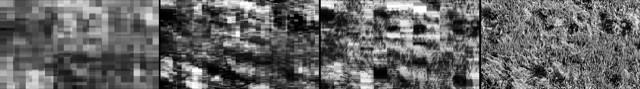
\includegraphics[width=\linewidth]{img/final/Mongrel_weed_4pr_row_ELISK_monoC}
  %%\caption{Screen dumps from the introduction of Machinic Propositions.}
\end{figure}

\begin{figure}\label{fig:impro-1}
  \centering
  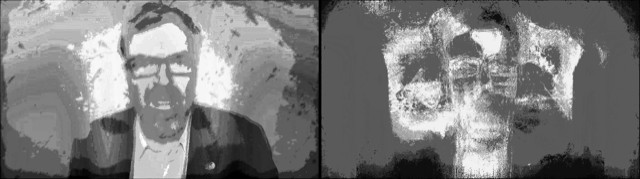
\includegraphics[width=\linewidth]{img/final/Mongrel_ansigLyd_2pr_row_ELISK_monoC_copy}
  %%\caption{Screen dumps from the introduction of Machinic Propositions.}
\end{figure}
\section*{Introduction}
\label{sec:introduction}

One\footnote{All images in this text are screen dumps from
  the latest version of Machinic Propositions, an intermedia work and
  ongoing project by
  the authors.} of the great promises of artistic research is the way in which it
allows for an insight into the inner workings of artistic
practices. Given an appropriate methodology, the researcher may tap
into the artistic processes or into the actual
performance itself. Although other research fields, such as art history,
musicology, ethnography, along with many others, have also shed light
on some of the processes behind artistic production, what makes
artistic research both challenging and interesting is the double role
played by researchers/artists. In part due to this special condition in artistic research or research focused
on artistic practices, it is not uncommon that the research also
introduces a change both into the practice and in the
artist/researcher. In fact, this may be seen as one of its features
\citep[][p. 27]{frisk-ost13}.

That changes in the processes that lead up to an artistic work may
change the outcome may not come as a surprise. What is remarkable,
however, is the extent to which the artistic
\emph{work} in Western culture is still often seen as an immutable
object and the product of one single originator. Even
relatively distributed artistic practices such as film production is
often referred to as the work of a director. The perspective of the
originator is guiding the apprehension of, and also, to some extent,
the understanding of the work of art. The points of reference in this
view are the stage 
director at the theatre (rather than the actors), and the composers
(rather than the musicians that play their music). For other fields, the configuration of the
agents involved may be of a different kind, but the dominance of the 
artwork to which a single originator may be attached is not to
be mistaken, especially in music.

There are, however, several indications that this view is slowly
changing. In 2005, with reference to Lydia Goehr's important work
\emph{The Imaginary Museum of Musical Works}, Georgina Born theorized
the changing ontology of music that opens up for ``an approach that
incorporates understandings of the social, technological and temporal
dimensions of music'' \citep[p. 8]{Born2005}. She points to several
important aspects of this development relating to, among other things,
the destabilizing effect that music in itself may have on common
dualisms such as subject/object and production/reception. This
resonates well with some of the ideas proposed in this short
text. Through artistic practice and consistent artistic methodology, the rigid conceptualization of music as an object rather than an activity may be questioned.


\section*{Machinic Propositions}
\label{sec:mongrel}

The duo \emph{Mongrel} has worked for several years on
numerous intermedia projects with the overarching ambition to critically
examine the nature of the relationship between auditory and visual
elements in intermedia works. Our works have been performed in the
United Kingdom, Denmark, Sweden, France, Belgium, Germany, and
Vietnam. \emph{Machinic propositions}, a project that we started in
2015 is simultaneously an artistic project and an attempt to critically examine Deleuze and
Guattari's theorems of deterritorialization as found in chapter seven
and ten of their seminal work \emph{A Thousand Plateaus}
\citep{deleuze80}. The output has taken a few different shapes and
has used different kinds of media such as text, live
performance and fixed media
format. Like much of our other works \emph{Machinic propositions} is
part of the attempt to counteract the predominance of one medium over
the other, in particular, video over audio. This is not to say that we necessarily
strive for their integration into one another. Instead the ambition
is to allow one to become the other under certain conditions,
comparable to what is described by Deleuze as ``not an exchange, but
'a confidence with no possible interlocutor' [\ldots]; in short, a
conversation'' \citep[p. 2]{deleuze77}.

Furthermore, there are parallels between the way we work,
and the idea put forward by Deleuze, of style as the ability to
``stammer in one's own language'' \citep[p. 3]{deleuze77}. Our working
process is, like any other artistic process, situated in our personal conditions and
flaws, but in \emph{Machinic Propositions} we use them to
gain access to the ability, discussed by Deleuze, to stammer in
language while avoiding it in speech \citet[p. 3]{deleuze77}. Among other things, we weave in Elberling's dyslexia and use his misreading of
the text as concrete material in the process allowing new meanings to rise from the mistakes.

\begin{figure}\label{fig:impro-1}
  \centering
  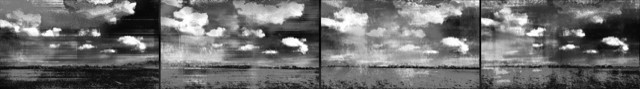
\includegraphics[width=\linewidth]{img/final/Mongrel_landskab_4pr_row_ELISK_monoC}
  %%\caption{Screen dumps from the introduction of Machinic Propositions.}
\end{figure}

In this project, we have looked at the
relation between the two media as a system of
de/re-territorialization. This has allowed us to
depart from some existing theories of sound and moving pictures, such as the
empathetic/anempathetic distinction proposed by
\citet{Chion1994}. Instead we have
attempted to detach both sound and image from their highly defined modes
of engagement. We examined the ways in which the
actual relations could be re-established within our systems of working,
using a range of approaches. One way through which we experimented with
these issues was to change roles in the work and performance
situation. Although we have our specific fields of competences, Frisk
centered on sound and Elberling on video, we decided to 
change roles so that Frisk was in charge of the video and vice
versa. As a result the attitudes towards the
material obviously changed. To some extent, this is a question
of creating usable interfaces for one another which in and of itself
provokes a rethinking of one's practice. In this case the actual
situation also changed our respective understanding of our practices
consistent with the core ambition to
deconstruct the relationship between sound and image.

Concerning the theorems of deterritorialization, there are some
interesting and immediate observations that may be done relating both
to the challenges in combining audio and video in general, as well as to our
particular practice. For instance theorem two quite literally has
some bearing on the factual reality of digital sound and image: ``The
fastest of two elements or movements of deterritorialization is not
necessarily the most intense or most deterritorialized.''
\citep[p. 193]{deleuze80} The update rate of digital audio and video
is in the region of 1764/1,\footnote{This obviously depends on the
  sample rate and the frame rate respectively but as a
  comparison audio is sampled 44100 times per second and the typical
  frame rate of video is 25fps.} yet video is commonly the dominant medium
in this relation.

Our practice, like many other
practices, may be likened to a rhizome, a network of ideas
that in the beginning is spread out on a plane. The nodes representing these ideas are highly distributed
in both space and time and appears to be unorganized. Eventually, through the work processes and the
conceptual development, a folding of this space is taking place, and
virtual wormholes are created. Nodes that in the beginning may
have been located far from each other may now be situated in
close proximity. This is to some extent a self-organizing process that finds
some resonance in \emph{A Thousand Plateaus}. In the opening chapter, by reference to
\citet{rosenstiehl974}, \citeauthor{deleuze80} comment that to:

\begin{quote}
  these centered systems, the authors contrast acentered systems,
  finite networks of automata in which communication runs from any
  neighbor to any other, the stems or channels do not preexist, and
  all individuals are interchangeable, defined only by their state at
  a given moment—-such that the local operations are coordinated and
  the final, global result synchronized without a central
  agency. \citep[p. 19]{deleuze80}
\end{quote}

\begin{figure}\label{fig:impro-1}
  \centering
  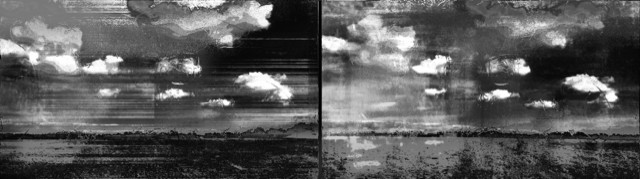
\includegraphics[width=\linewidth]{img/final/Mongrel_landskab_2pr_row_ELISK_monoC}
\end{figure}

Artistic work is to some extent a practice that takes
place in material reality, even if the perception of such actions may
approach the virtual. In music, the
practice often needs time to develop--although some processes are
better developed out of time. Nevertheless, the way Deleuze and
Guattari talk about the rhizome as ``a map and not a tracing''
\citep[p. 13]{deleuze80} is, at least for the work method we have
developed, both a fitting description and a useful mode with which to further
develop our processes. Mapping the patterns we are creating, our
individual as well as each other's, is a process that may be
seen as the attempt to reduce the number of possibilities in our
project, while at the same time attempt to increase the number of
possible connections. Just
before we engaged in the work on \emph{Machinic Propositions} we wrote
in our work journal that ``the solution lies rather in the attempt to
move away from trying to synchronize the perception of sound and
video, and instead focus on common processes that bind the elements
together.''\footnote{Project diary, translated from Swedish by the
  authors, March 11, 2015. } In other words, it is not how we attempt
to synchronize the mediums with each other but rather how the
activities that construct these mediums in the first place.

Through the theorems of \emph{A Thousand Plateaus} we began to work
out an abstract intermedial work trying to maintain a critical
attitude towards the philosophy of Deleuze and Guattari specifically,
and the very notion of using philosophy as the input to artistic
processes in general. With the use of the theory, we further developed our
conceptual tools, and more specifically, the way we used our senses
\emph{to see} and \emph{to hear} in the way we tackled the theory.
Together this participated in creating a zone of relative freedom that may provide
possibilities for a new understanding of what we do as artists and
researchers.

\begin{figure}\label{fig:impro-1}
  \centering
  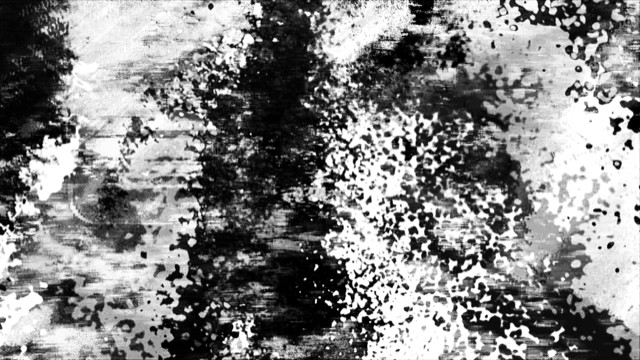
\includegraphics[width=\linewidth]{img/final/Mongrel_double_vindow_feed_1pr_row_ELISK_monoC}
  %%\caption{Screen dumps from an image transformation in Machinic Propositions.}
\end{figure}

\section*{Conceptual deduction}
\label{sec:conceptual-deduction}

Our artistic method is one where narrative and improvisation play central
roles. It has grown out of our thinking about contemporary media and
our attempts to critically examine both our own pro-technical
approach, and the hypermedia landscape we act and live in. The method has
been developed based on our artistic ideas, the needs of the projects
we engage in, and the conditions of our respective practices. Our process is slow
and meticulous. The work on \emph{Machinic propositions} began in 2015
and is likely to continue for another few years. In other words, what
is commonly seen as the
actual artwork--the work in performance--only materializes at the very end of a relatively long
process of interaction. Furthermore, in our method, it may continue to develop
through numerous iterations long after that. However, the work in itself in terms of a
resulting performance is in this
context less important than the process, to the point where there is
almost a reversal of the two terms: the \emph{work} is the process and the
actual performance work is simply one out of many possible parts of the process. 

The method of conceptual deduction is related to a variety of contexts
and may primarily be associated with scientific research and
systematic inquiry perhaps not commonly referenced in the context of
artistic research. In Monrad Rrenban's book on the early works of
Walter Benjamin, he writes that ``Benjamin suggests the practice of
philosophy is not the conceptual deduction (deduction into concepts)
of research but is also somewhat distinct from the metaphorical
determinateness [\ldots] in the artwork''
\citep[p. 117]{rrenban2005}. For us, however, both the metaphorical
determinateness and the conceptual deductions are part of the
formative movement towards a performance. In \emph{Mongrel} we are
using it freely, and mainly as a tool to reason our way through the
constructive phases of our artistic practice. In some ways, this is
not so different from using improvisation as a method as improvisation
may also be concerned with the creation of models that contribute to
bringing the negotiation of material forward. Hence, it is a process
in which we align and synchronize the general ambition of the work
and, perhaps most importantly, it brings differences in our respective
aesthetics to the surface in a way that is useful to us. We may start
with an existing story, a fictional character or a philosophical text,
but we may end up with something quite different. Being as it is
artistic practice, the goal of the method is to create a
performative platform that we share and that we later use to guide the
development of material for our works.

It is a time-consuming process the strength of which is not always
evident in the practice and it can lead to the kind of pivotal moments
where the entire structure needs to be rethought. As was mentioned,
the basic premise of the method, the way we use it, is that we start
with a general story or concept that we explore together.

\section*{Discussion}
\label{sec:discussion}

Part of our method is to improvise in the studio, both as a means for
generating material and for evaluating the effectiveness of the
performance situation. In these recorded sessions the impact of the
listening position is sometimes quite obvious. For example, the
immediate memory of the quality of the playing may be that it was
highly consistent. Listening back to it at a later time, however, the
impression of the performance may be rather different such that
several edits are necessary for it to work. In this project we have
discussed this phenomenon as a process of deterritorialization; the
improvisation taking place in real time is deterritorialized into a
hybrid composition in fixed time and a composition affords a different
kind of listening than an improvisation. 

Ellestrom comments that ``the understanding of what
a medium is and what intermedial relations actually consist of has
vital implications for each and every inquiry in old and new fields of
study concerning the arts and media: ekphrasis, cinema, illustration,
visual poetry, remediation, adaptation, multimedia and so on''
\citep[p. 11]{Ellestrom2010}. Unless we attempt to understand the
underlying processes that come into play when an improvisation is
recorded and then listened back to, we cannot use the information we
get from listening to the recording in a way that contributes to
our work. This process is similar to what is described
in \emph{theorem five}:
\begin{quote}
  deterritorialization is always double, because it implies the
  coexistence of a major variable and a minor variable in simultaneous
  becoming (the two terms of a becoming do not exchange places, there
  is no identification between them, they are instead drawn into an
  asymmetrical block in which both change to the same extent, and
  which constitutes their zone of proximity). \citep[p. 338]{deleuze80}
\end{quote}
The music, first improvised and then recorded, becomes a double
articulation and the content in both contexts changes to a
degree where neither may be understood in the way they could prior to
the deterritorialization. The recording
expropriates the content transforming it from the original
improvisation and it \emph{becomes} a composition.

\begin{figure}\label{fig:impro-1}
  \centering
  
\includegraphics[width=\linewidth]{img/final/Mongrel_mist_2pr_row_ELISK_monoC}
\end{figure}

The continuous iterations of
practice-reflection feedback loops and, along with them, the
theory-method interactions that may surface as a result, are among
some of the most interesting aspects of artistic research. These
may involve de/reterritorializing the borders between preparation and
performance, between design time and play time and between different
media. In these lines or blocks of becoming there is an opening for a radical
and experimental research practice that has social as well as
political connotations, but most of all it contributes to our artistic practice.

For the musician to understand and go beyond the
the differences between the modes of listening to the development of
material, and the complimentary listening to the result of the same
process, may be second nature. Partly, artistic research is the
attempt to extract the implications of the knowledge development in those
and similar processes, collect the data, and then
go back and develop the musical possibilities allowed for with the new
information. But also to attempt to understand the results outside of the field of artistic practices.
In this sense, artistic
research is interdisciplinary, transformative and deterritorializing. It opens up new perspectives on the roles
of the various agents in the field of performance such as the
audience, the sociocultural contexts and many other. Even though the history of
art practice is full of examples of practitioners that have worked in
this very manner, and as a consequence, this aspect of artistic
research is not unique or new. However, the transformative aspect of artistic
research should attempt to continuously move the borders of what is
possible; in art as well as in research.


\printbibliography
% Emacs 24.5.1 (Org mode 8.2.5h)
\end{document}
